\scalebox{0.9}{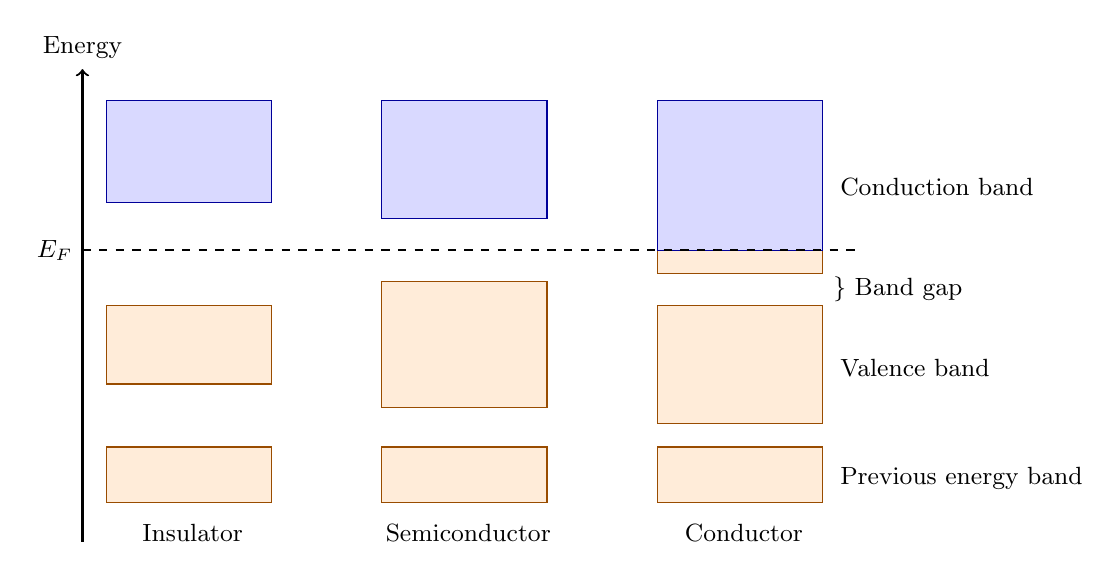
\begin{tikzpicture}[font=\small]

  % ── parameters ──────────────────────────────────────────────────
  \def\bw{2.2}   % band width

  % x-centres of the three columns
  \def\xIns{0}
  \def\xSemi{3.5}
  \def\xCond{7}

  % Fermi level y
  \def\yFermi{3.2}

  % ── INSULATOR ───────────────────────────────────────────────────
  % previous band
  \fill[orange!15] (-1.1, 0) rectangle (1, 0.7);
  \draw[orange!60!black] (-1.1, 0) rectangle (1, 0.7);

  % valence band
  \fill[orange!15] (-1.1, 1.5) rectangle (1, 2.5);
  \draw[orange!60!black] (-1.1, 1.5) rectangle (1, 2.5);

  % conduction band
  \fill[blue!15] (-1.1, 3.8) rectangle (1, 5.1);
  \draw[blue!60!black] (-1.1, 3.8) rectangle (1, 5.1);

  \node[below] at (\xIns, -0.15) {Insulator};

  % ── SEMICONDUCTOR ───────────────────────────────────────────────
  % previous band
  \fill[orange!15] (2.4, 0) rectangle (4.5, 0.7);
  \draw[orange!60!black] (2.4, 0) rectangle (4.5, 0.7);

  % valence band
  \fill[orange!15] (2.4, 1.2) rectangle (4.5, 2.8);
  \draw[orange!60!black] (2.4, 1.2) rectangle (4.5, 2.8);

  % conduction band
  \fill[blue!15] (2.4, 3.6) rectangle (4.5, 5.1);
  \draw[blue!60!black] (2.4, 3.6) rectangle (4.5, 5.1);

  \node[below] at (\xSemi, -0.15) {Semiconductor};

  % ── CONDUCTOR ───────────────────────────────────────────────────
  % previous band
  \fill[orange!15] (5.9, 0) rectangle (8, 0.7);
  \draw[orange!60!black] (5.9, 0) rectangle (8, 0.7);

  % valence band
  \fill[orange!15] (5.9, 1) rectangle (8, 2.5);
  \draw[orange!60!black] (5.9, 1) rectangle (8, 2.5);

  % conduction band
  \fill[orange!15] (5.9, 2.9) rectangle (8, \yFermi);
  \draw[orange!60!black] (5.9, 2.9) rectangle (8, \yFermi);

  \fill[blue!15] (5.9, \yFermi) rectangle (8, 5.1);
  \draw[blue!60!black] (5.9, \yFermi) rectangle (8, 5.1);

  \node[below] at (\xCond, -0.15) {Conductor};

  % ── FERMI LEVEL dashed line ──────────────────────────────────────
  \draw[dashed, thick] (-\bw/2 - 0.3, \yFermi) -- (\xCond+1.5, \yFermi);
  \node[left] at (-\bw/2 - 0.3, \yFermi) {$E_F$};

  % ── BAND-GAP manual bracket (conductor column) ───────────────────
  \node[right=2pt] at (\xCond+\bw/2-0.2, 2.7) {$\left. \right\}$ Band gap};

  % ── RIGHT-SIDE LABELS ────────────────────────────────────────────
  \node[right] at (\xCond+\bw/2, 4) {Conduction band};
  \node[right] at (\xCond+\bw/2, 1.7)  {Valence band};
  \node[right] at (\xCond+\bw/2, 0.3)  {Previous energy band};

  % ── ENERGY AXIS ──────────────────────────────────────────────────
  \draw[->, thick] (-1.4, -0.5) -- (-1.4, 5.5) node[above] {Energy};

\end{tikzpicture}}